In this thesis, partial state is implemented in Noria~\cite{noria}, a stateful,
dynamic, parallel, and distributed dataflow system designed for the storage,
query processing, and caching needs of typical web applications. Because of the
strong connection between Noria and partial state, this chapter describes the
design and implementation of Noria in sufficient depth to understand the
remainder of the thesis.

\section{High-Level Overview}

Noria runs on one or more multi-core servers that communicate with clients and
with one another using RPCs. A Noria deployment stores both \emph{base tables}
and \emph{derived views}. Roughly, base tables contain the data typically stored
persistently in relation tables, and derived views hold data an application
might choose to cache to improve performance.

Compared to conventional database use, Noria base tables might be smaller, as
Noria derives data that an application may otherwise precompute and store
denormalized in base tables for performance. Noria stores base tables
persistently on disk, either on one server or sharded across multiple servers.
Views, by contrast, are likely larger than a typical cache footprint, because
Noria derives more data, including some intermediate results. Noria stores views
in memory.

Noria's interface resembles parameterized SQL queries. The application supplies
a \emph{Noria program}, which registers base tables and views with parameters
supplied by the application when it retrieves data. The Noria program includes
base table definitions, \emph{internal} views used as shorthands in other
expressions, and \emph{external} views that the application later queries
(the next section gives an example). It can be thought of as an extended schema
for the application that includes its queries.

Noria differs substantially from traditional databases in how it executes
queries. Rather than compute a query's results on demand when the application
executes it, Noria does so when the query view is defined. Noria then caches, or
\emph{materializes}, the contents of that view, and serves queries to that view
directly from that cache. To keep the materialized view current, Noria
internally instantiates a dataflow program to continuously process the
application's writes and update the views as appropriate.

This kind of view materialization makes Noria well-suited for read-heavy
applications that tolerate eventual consistency, since it shifts query execution
cost from reads, which are frequent, to writes, which are infrequent.

\paragraph{Materialization.}
Throughout this thesis, the word materialization is often used as a noun. In the
context of Noria, a materialization refers to any derived computation result
that Noria explicitly stores, not just materialized views. Or, more precisely,
Noria may choose to materialize intermediate results, such as the current value
of an aggregation, which do not represent any of the application's queries.
These intermediate materializations are still views\,---\,they have a schema and
consist of rows\,---\,but do not reflect any named views that the application
has created.

\section{Application Interface}

\begin{listing}[h]
  \begin{minted}{sql}
/* base tables */
CREATE TABLE stories (id int, title text);
CREATE TABLE votes (story_id int, user int);
/* internal view: vote count per story  */
CREATE INTERNAL VIEW VoteCount AS
  SELECT story_id, COUNT(*) AS vcount
    FROM votes GROUP BY story_id;
/* external view: story details */
CREATE VIEW StoriesWithVC AS
  SELECT id, author, title, url, vcount
    FROM stories
    JOIN VoteCount ON VoteCount.story_id = stories.id
   WHERE stories.id = ?;
  \end{minted}
  \caption{Noria program for a key subset of the Lobsters news
           aggregator~\cite{lobsters} that counts users' votes for stories.}
  \label{l:vote-src}
\end{listing}

Listing~\vref{l:vote-src} shows an example Noria program for a news aggregator
application where users can vote for stories.

To retrieve data, the application supplies Noria with an external view
identifier (e.g., \texttt{StoriesWithVC}) and one or more sets of parameter
values (\texttt{?} is a parameter). Noria then responds with the records in the
view that match those values. To modify records in base tables, the application
performs insertions, updates, and deletions, similar to a SQL database. Data is
represented as structured records in tabular form~\cite{spanner, bigtable}.

The application may change its Noria program to add new views, to modify or
remove existing views, and to adapt base table schemas. When it does, Noria
adapts the running dataflow to incorporate the changes without restarting the
dataflow engine.

Unlike the iterative or graph computations that are the focus of other dataflow
systems~\cite{naiad, differential-dataflow}, Noria focuses entirely on
relational operators. Noria supports much, but not all, SQL.

\section{Dataflow Execution}

To keep its materialized views from growing stale as the underlying data
changes, Noria uses dataflow. Noria compiles all the application queries into a
joint dataflow program, which it routes all application writes through. The
dataflow is a directed acyclic graph of relational operators such as
aggregations, joins, and filters. Base tables are the roots of this graph, and
external views form the leaves. Noria extends the graph with new base tables,
operators, and views as the application adds new queries.

When an application write arrives, Noria stores it in a base table and then
injects it into the dataflow as an \emph{update}. Operators process the update
and emit derived updates to their children. Eventually, updates reach and modify
the external views. Updates are \emph{deltas}~\cite{roll, differential-dataflow}
that add to, and remove from downstream state. Deltas are similar to
mathematical multisets, or ``bags'', except that the multiplicity of an element
may be negative.

As an example, a count operator emits deltas that indicate how the count for a
key has changed; a join may emit an update that installs new rows in downstream
state; and a deletion from a base table generates a ``negative'' update that
revokes derived records. Negative updates remove entries when Noria applies them
to state, and retain their negative ``sign'' when combined with other records
(e.g., through joins). Negative updates hold exactly the same values as the
positives they revoke and follow the same dataflow paths.

The combined deltas an operator emits from the beginning of time constitutes the
operator's current state. This state may be entirely virtual, or the delta
stream may be \textit{materialized}, in which case the current multiset of
records is stored by the system. It is helpful to think of \emph{edges} as being
materialized, rather than operators or views, since a materialization is exactly
equivalent to the evaluation of the deltas that have flowed across that edge.

Noria supports \emph{stateless} and \emph{stateful} operators. Stateless
operators, such as filters and projections, need no state to process updates;
stateful operators, such as count, min/max, and top-$k$, maintain state to avoid
inefficient re-computation of aggregate values from scratch. Stateful operators
also keep one or more indexes to speed up operation. Noria adds indexes based on
\emph{indexing obligations} imposed by operator semantics; for example, an
operator that aggregates votes by user ID requires a user ID index to process
new votes efficiently. Noria's joins are stateless, but require that the state
of their inputs be materialized to allow an update arriving at one input to join
with all relevant state from the other.

Noria always processes updates in order along any given dataflow edge, but
chooses non-deterministically among different input edges which one to process
updates from next.

\subsection*{Example Execution}

\begin{figure}[t]
  \centering
  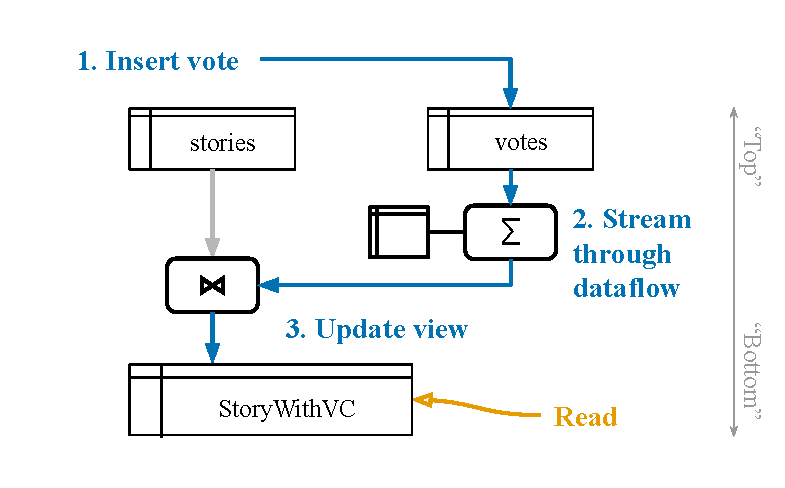
\includegraphics{diagrams/Example Execution.pdf}
  \caption{Noria's dataflow program to maintain Listing~\ref{l:vote-src}. Text
  describes the update path highlighted in \textbf{\color{set1}blue}. The
  dataflow inputs are considered the ``top'' of the dataflow, and the leaves are
  at the ``bottom''. Parents are ``upstream'' of their ``downstream'' children.}
  \label{f:example-exec}
\end{figure}

Figure~\vref{f:example-exec} shows the dataflow that Noria constructs for
maintaining the Noria program in Listing~\vref{l:vote-src}. At the top are the
entry points into the dataflow\,---\,the operators that represent the schema
base tables\,---\,one for the \texttt{stories} table, and one for the
\texttt{votes} table. Connected to the \texttt{votes} table is a counting
aggregation operator ($\sum$), which corresponds to the internal
\texttt{VoteCount} view. It feeds into a join operator ($\bowtie$), which in
turn connects to the external \texttt{StoryWithVC} view.

To understand how Noria uses this program to maintain the external view,
consider what happens when the application adds a new vote. The application
performs the insertion by introducing the write into the dataflow as a
single-row update with a positive sign at the \texttt{votes} operator. Noria
stores the update to durable storage, and then forwards the update as-is to its
children; in this case, the count operator.

The count operator performs a lookup into its own output state for the current
count of the new row's group by column value. The semantics of a count is that
an insertion increments that number by one, so the operator emits a replacement
update for the old state. In particular, the update it produces contains a
negatively-signed delta with the old count, and a positively-signed delta with
the updated count. Both deltas include the group by column value.

The replacement is represented as a separate negative and positive delta since
the two may take different paths through the dataflow. For example, a downstream
filter might filter out stories with a vote count below a given threshold. If
the latest vote makes the count exceed the threshold, the negative delta should
not flow down the dataflow past the filter, since there is nothing there for it
to revoke. However, the positive delta should, since the story (with its updated
count) now passes the filter.

When the join receives this replacement update from the count, it looks in its
other ancestor, \texttt{stories}, for records that match the join column value
of each delta of the incoming update. In this case, both deltas (the negative
one and the positive one) have the same story identifier as the join value, and
the lookup finds only a single record\,---\,the matching story. The operator
then joins each delta with each matching result. This produces an update that
(still) contains one negative and one positive delta, but where each delta now
includes additional columns from the \texttt{stories} table.

Ultimately, this two-delta update arrives at the operator that represents the
external \texttt{StoryWithVC} view. The changes from the update are applied one
by one, with the negative delta removing the entry in the view with the old vote
count, and the positive delta adding the replacement entry.

\section{Consistency Semantics}
\label{s:noria:consistency}

To achieve high parallel processing performance, Noria's dataflow avoids
global progress tracking or coordination. An update injected at a base table
takes time to propagate through the dataflow, and the update may appear in
different views at different times. Noria operators and the contents of its
external views are thus \emph{eventually-consistent}: if writes quiesce,
external views eventually hold results that are the same as if the queries were
executed directly against the base table data at a single point in time.
Eventual consistency is attractive for performance and scalability, and is
sufficient for many web applications~\cite{eventually-consistent,
facebook-memcache, pnuts}.

% In the meantime

Eventual consistency is an inherently vague consistency model\,---\,an
eventually consistent system may return incorrect results as long as it
\emph{eventually} returns the right result. In practice, eventual consistency is
often ``good enough'' despite giving few \emph{guarantees}, and many eventually
consistent systems appear strongly consistent most of the time~\cite{eventual}.

Ensuring even this relatively weak property requires some care. Like most
dataflow systems, Noria requires that operators are \textbf{deterministic}
functions over their own state and the inputs from their ancestors. Furthermore,
operators must be \textbf{distributive over delta addition}\footnote{$d_1 + d_2$
produces the union of all rows in $d_1$ or $d_2$ with the signed multiplicity of
each row equal to the algebraic sum of that row's signed multiplicity in $d_1$
and $d_2$.} so that evaluating the query using tuple-at-a-time processing is
equivalent to evaluating the whole query at once. Finally, Noria operators must
be \textbf{commutative} so that operators with multiple inputs, like unions and
joins, can process their inputs in any order without
coordination\footnote{Eventual consistency with partial state requires
additional mechanisms (\S\ref{s:correct}).}. The standard relational operators
that Noria supports all have this property.

\paragraph{How Eventual?}
While Noria does not guarantee when a write is visible in a given view, the time
between when a write is acknowledged and when it becomes visible is not
completely arbitrary. A view is stale only while the write propagates through
the dataflow, so the time before the write manifests depends only on the height
and complexity of the dataflow for the view in question. While eventual
consistency allows reads to give arbitrary results until they \emph{eventually}
return the correct result, Noria reads are generally just stale.

\subsection{What Can Go Wrong?}

Noria's eventual consistency can lead to reads giving strange results under
certain circumstances in stream processing systems~\cite{materialize-eventual}.
This subsection covers a number of such cases.

\paragraph{View Discrepancy.}
If a client reads from view $V_1$ and then from view $V_2$, the read from $V_2$
may reflect changes that are not yet visible in $V_1$. For example, if a client
inserts row $r$ into base table $A$, $r$ may appear in $V_1$ without yet
appearing in $V_2$, or vice-versa. Similarly, if view $V$ is sharded, and a
client reads from two different shards, either read may reflect changes that are
not reflected in the other.

\paragraph{Incomplete Effects.}
A client that reads form view $V$ may observe \emph{some} of the effects of a
base table change, like an insert, but not others. This occurs if the dataflow
that maintains $V$ contains a diamond\,---\,a fork followed later by a merge
operator like a union or join. The dataflow update that results from an insert
into a base table is processed by one ``side'' of the diamond before the other,
and in the intervening time the view reflects only the effects from that
dataflow path. Indeed, if one path is much slower than the other, multiple base
table changes may flow through the fast path, and be reflected in $V$, before
\emph{any} effects from the other path manifest.

\paragraph{Independent Writes.}
If a client writes to a base table $A$, and then to a different base table $B$,
and then reads from a view $V$ that is downstream of both $A$ and $B$, it may
see the effects of only the write to $B$ reflected in $V$. For example, if $A$
is a table of albums, and $B$ is a table of images, a client that creates an
albums and adds an image to it may briefly see the image appear with no
associated album.

\begin{listing}[h]
  \begin{minted}{sql}
    SELECT data.key FROM data
    WHERE data.value IN
      (SELECT MAX(data.value) FROM data)
  \end{minted}
  \caption{Query that may perpetually produce no results in Noria.}
  \label{l:always-wrong}
\end{listing}

\paragraph{Unsynchronized Joins.}
Consider the query in Listing~\vref{l:always-wrong}. If the maximum value
changes frequently enough, then the outer and inner query may be perpetually
``out-of-sync''. The current maximum may not yet be present in the outer query,
or a new maximum value may not yet be present in the inner query. The net result
is that the result set of the query would be empty, even though a traditional
database would never yield an empty query result. If the max value changes less
frequently, and Noria has time to process a new update through both dataflow
paths (the inner and the outer) before the maximum changes again, Noria will
produce the expected non-empty query result.

\subsection{Why Does It Go Wrong?}

Exactly how strange these phenomena become, and how often they manifest, depends
on the nature of the queries and the updates. For example, queries that access
each base table only once produce results that are stale, but never results that
do not match the results a traditional database would have given given the same
base table data. Queries with self-joins on the other hand are particularly
prone to these temporary inconsistencies. For example, a join that computes a
parent-child relationship between records may briefly reflect a new record as a
child, but not as a parent, or vice-versa.

This is all because these inconsistencies arise due to race conditions in the
dataflow graph. In particular, if two deltas resulting from a single upstream
change race against each another down different dataflow paths that later
converge, one delta will be applied to the final view before the other. This
leaves the view in an intermediate state where a partial effect of the original
update can be observed until the other delta arrives.

\begin{listing}[h]
  \begin{minted}{sql}
    SELECT id, state FROM data WHERE state = 1
    UNION
    SELECT id, state FROM data WHERE state = 2
  \end{minted}
  \caption{Query that may produce duplicates briefly in Noria.}
  \label{l:duplicates}
\end{listing}

Listing~\vref{l:duplicates} gives an example of a query with this kind of race
condition. Imagine that the application changes the \texttt{state} where
\texttt{id = 42} from 1 to 2. In Noria, this is represented by a removal of the
now-outdated record, and an addition of the updated record. The removal follows
the dataflow path for \texttt{WHERE state = 1}, while the addition follows the
dataflow path for \texttt{WHERE state = 2}. One of those updates will arrive
first at the union, and the materialized view. If it is the removal, then reads
will not see a record with \texttt{id = 42} until the addition is processed.
Conversely, if the addition arrives first, reads will see two records with
\texttt{id = 42} (one with \texttt{state = 1} and one with \texttt{state = 2})
until the removal is processed.

A query that accesses each dataflow only once never makes an update race ``with
itself'', and thus never produces intermediate output, only stale output. A
self-join on the other hand frequently makes updates resulting from one base
table change race, and can therefore exhibit these ``strange'' results.

To mitigate these kinds of inconsistencies, Noria would either need to enforce
that no reads can happen between the application of one ``half'' and the other,
or somehow hide the partial effects of applying only the first part. The former
requires reads to flow through the dataflow, or at least synchronize closely
with it, which would likely come at a penalty to read latency. The latter would
be provided through something akin to multi-version concurrency control, which
allows low-latency reads, but adds significant system complexity.

Instead, Noria works under the assumption that queries that produce these
inconsistencies are rare for Noria's target applications, or that application
developers direct those queries where strong consistency is necessary to other,
better suited systems.

\section{Parallelism}
\label{s:parallel}

Servers have many cores, and high-performance systems must use these cores to
take full advantage of the hardware. Noria does so in several ways. First, it
allows reads to happen independently from any number of threads concurrently.
Second, it allows different threads to process writes in disjoint parts of the
dataflow concurrently. And third, it supports sharding individual operators, or
cliques of operators, so that multiple threads can process disjoint subsets of
the data concurrently through the same dataflow segment. These three mechanisms
are described further below.

\subsection{Read Independence}

Since Noria is designed for read-heavy workloads, its architecture is optimized
to allow reads to go ahead at full speed whenever possible. In particular, Noria
does not synchronize reads with reads \emph{or} writes\footnote{If a read
encounters missing partial state, as described in the next chapter, some
lightweight synchronization is needed to communicate the missed key}.

This is achieved through a concurrency primitive that maintains two instances of
each materialized view, with deduplication between them. Reads go to one view,
and writes to the other. Readers see updates to the view only when a writer
exposes those changes explicitly\,---\,the writer flips an atomic pointer to the
other view, and then waits for all readers to exit the old view before modifying
it again. This flip can be done on every update, as Noria currently does, or
only occasionally to amortize the cross-core communication penalty and the wait
period for the writer. Crucially, readers do not take locks, and generally
operate only on core-local cache lines.

This design allows Noria to use any number of threads to serve reads from any
view. As long as there are cores available, Noria can use additional threads to
perform view lookups, as well as low-level networking work like request
serialization and read/write system calls.

\subsection{Partitioning}
\label{s:noria:partitioning}

The dataflow model is inherently streaming, and thus well-suited for distributed
deployments. Operators are independent and communicate only through their
streams, so Noria can place them on different cores, or hosts, and use
appropriate messaging fabrics to connect them.

Tot take advantage of this, Noria divides the dataflow graph into a number of
sub-graphs called \textit{thread domains}. Only a single thread can process
updates in a given thread domain at a time (except with sharding; see below),
and any update that enters a thread domain is processed to completion within
the domain before another update is processed.

Noria never shares state between thread domains, which means that state access
is not guarded by locks. Thread domains communicate with one another only
through messages across the edges of the dataflow, or in the case of upqueries,
by sending messages through dedicated upquery paths set up by the partial
subsystem. All such communication can happen either over the network if the
other thread domain is on a different host, or over an in-memory channel if it
is local.

Since thread domains share nothing, Noria duplicates state across boundaries
when needed. For example, a join operator at an incoming edge of a thread domain
must be able to perform lookups into the state of its ancestor, which sits in a
different thread domain. In such a case, Noria will create a thread-local copy
of the join's ancestor's state that it can use locally. Noria's thread domain
assignment heuristics will attempt to draw domain boundaries  such that this
kind of duplication is unnecessary. For example, it will prefer drawing a domain
boundary just before an aggregation (which does not need to look up in the state
of its ancestor), and avoid drawing a domain boundary just before a join.

\subsubsection{Join Consistency}
\label{s:join-state-dupe}

The thread-local copy of lookup state, such as for joins, serves a second
purpose: it mitigates a race condition that would otherwise arise from
cross-domain state lookups. Consider a join operator J with parents L and R. If
R's state was in a different domain than J, then the following can happen:

\begin{enumerate}
  \item R receives and incorporates a delta $d_R$ that adds row $r_R$.
  \item J receives a delta $d_L$ from L that adds row $r_L$.
  \item J performs a lookup in R's state based on $d_L$'s join key. The result
    includes $r_R$, so J emits a delta that adds $r_L \bowtie r_R$.
  \item $d_R$ arrives at J.
  \item J performs a lookup in L's state based on $d_R$'s join key. The result
    includes $r_L$, so J emits a delta that adds $r_L \bowtie r_R$ a second
    time.
\end{enumerate}

This issue arises because the lookups bypass deltas in flight between R and J;
the lookups get to observe ``the future''. This erroneously causes J to
incorporate the same data at two points in time, which would lead to perpetually
incorrect results in the downstream views.

Multi-version concurrency control could likely be used to solve this problem,
but would be heavyweight solution that also requires much more significant
synchronization. Especially if J and R happen to be on different physical hosts.
Duplicating R's state across the domain boundary avoids the problem\,---\,since
thread domains process all updates within the domain to completion, there can be
no deltas in flight between R and J, and the lookup will never observe future
state.

\subsection{Sharding}
\label{s:noria:sharding}

To accommodate applications with such a high volume of writes that the
processing at a single operator is a bottleneck, Noria supports sharding an
operator. Multiple threads split the work of handling updates to a sharded
operator, and operate like independent, disjoint parts of the dataflow.

Noria implements static hash partitioning: it decides how to shard an operator
when the operator is added to the dataflow, and this sharding does not change
over the runtime of the application. Sharding by value ranges and adjusting the
sharding dynamically is left for future work.

Noria shards operators primarily based on how they access state. For example, an
aggregation that performs lookups into its own state is sharded by the key
column of those lookups. Any other sharding would mean that processing one
update would require coordination among all shards. A join is sharded by the
join key for the same reason. Base tables are sharded by the table's primary
key. Operators that do not perform lookups (e.g., unions) continue the sharding
of their ancestors to avoid unnecessary resharding.

To shard an operator, Noria introduces two additional nodes in the dataflow: a
\emph{sharder} placed upstream of the sharded operator, and a \emph{shard
merger} downstream of it. The sharder routes incoming updates to the appropriate
shard of the sharded operator, and the shard merger is a union operator that
combines the output of all the shards to a single downstream output stream.
Noria then eliminates unnecessary sharders and shard mergers, such as if an
operator and its ancestor are sharded the same way.

Sharding boundaries are also natural thread boundaries, though two connected
thread domains may also be sharded differently. Or, phrased differently, Noria
may partition a chain of operators that are all sharded by the same column into
multiple thread domains to increase parallelism.

% Sharding is tracked based on "ultimately source column". (column tracing)
